\begin{frame}{Геометрический изгиб дуг}

\begin{columns}
\begin{column}{0.65\textwidth}
Был исследован и разработан математический метод изгиба дуг, конфликтующих с другими объектами графа. Метод заключается в обособленном изгибе дуги в собственном базисе по средствам параметрического описания кривой, и перехода к изначальному базису системы графа, благодаря которому, кривая правильно позиционируется в пространстве.
\end{column}
\begin{column}{0.35\textwidth}
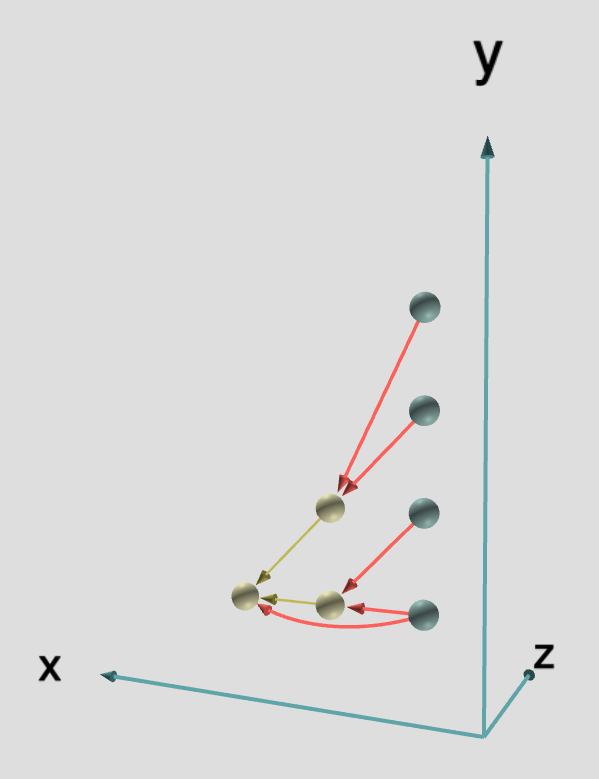
\includegraphics
[width=\textwidth]{images/example2}\\
\end{column}
\end{columns}

\end{frame}